In order to gain a deeper understanding of the physics learned by the CNN tagger, 
we examine how the internal structure of the network relates to the properties of
quark and gluon jets, following the strategy outlined in Ref.~\cite{deOliveira:2015xxd}.
Figure~\ref{fig:correlation} shows, for each pixel of the jet image, the Pearson Correlation Coefficient
of the pixel intensity with the final CNN tagger output.
The intensity of the four pixels at the core of the jet are strongly correlated with CNN tagger output and
are thus important to identify quark jets. The intensity of outer pixels in the jet image are instead anti-correlated with
the CNN tagger output, in agreement with the intutition that gluon jets tend to feature a wider radiation pattern.

The discriminating information extracted by each convolutional filter can also be investigated.
This is done by visualizing the average difference between the convolution of each filter with the input image for quark 
and gluon jets.
More formally, let $I_q$ and $I_g$ be the average quark and gluon jet images, respectively.
The average difference between the convolution of a filter $w_i$ is obtained by computing $I_q * w_i - I_g * w_i$, where $*$ represents the convolution operator.
The visualizations for the first convolutional layer of the CNN tagger are shown in Figure~\ref{fig:filters}.
As the images are not rotated prior to training, 
many of the filters are simply rotations of other filters.  Some of the filters show features that are readily interpretable in terms of physical notions such as the soft haze around a jet core, but others are more complex and require further study to understand.  

\begin{figure}[htbp]
\begin{center}
\subfloat[][]{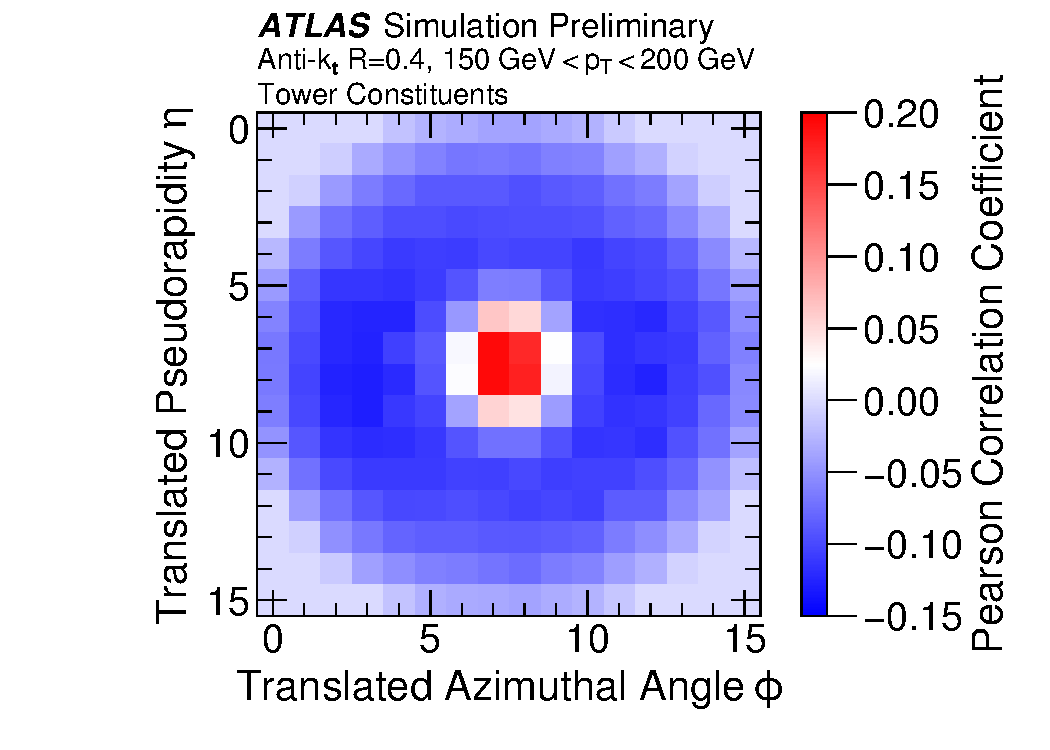
\includegraphics[width=0.5\textwidth]{figures/CNN/corr_tower150200.pdf}}
\caption{
Per-pixel linear correlation with CNN tagger output.
}
\label{fig:correlation}
\end{center}
\end{figure}

The visualizations in Figures~\ref{fig:correlation} and~\ref{fig:filters} are an important start to probing 
what the CNN is learning about the jet radiation pattern.  
 
\begin{figure}[htbp]
\begin{center}
\subfloat[][]{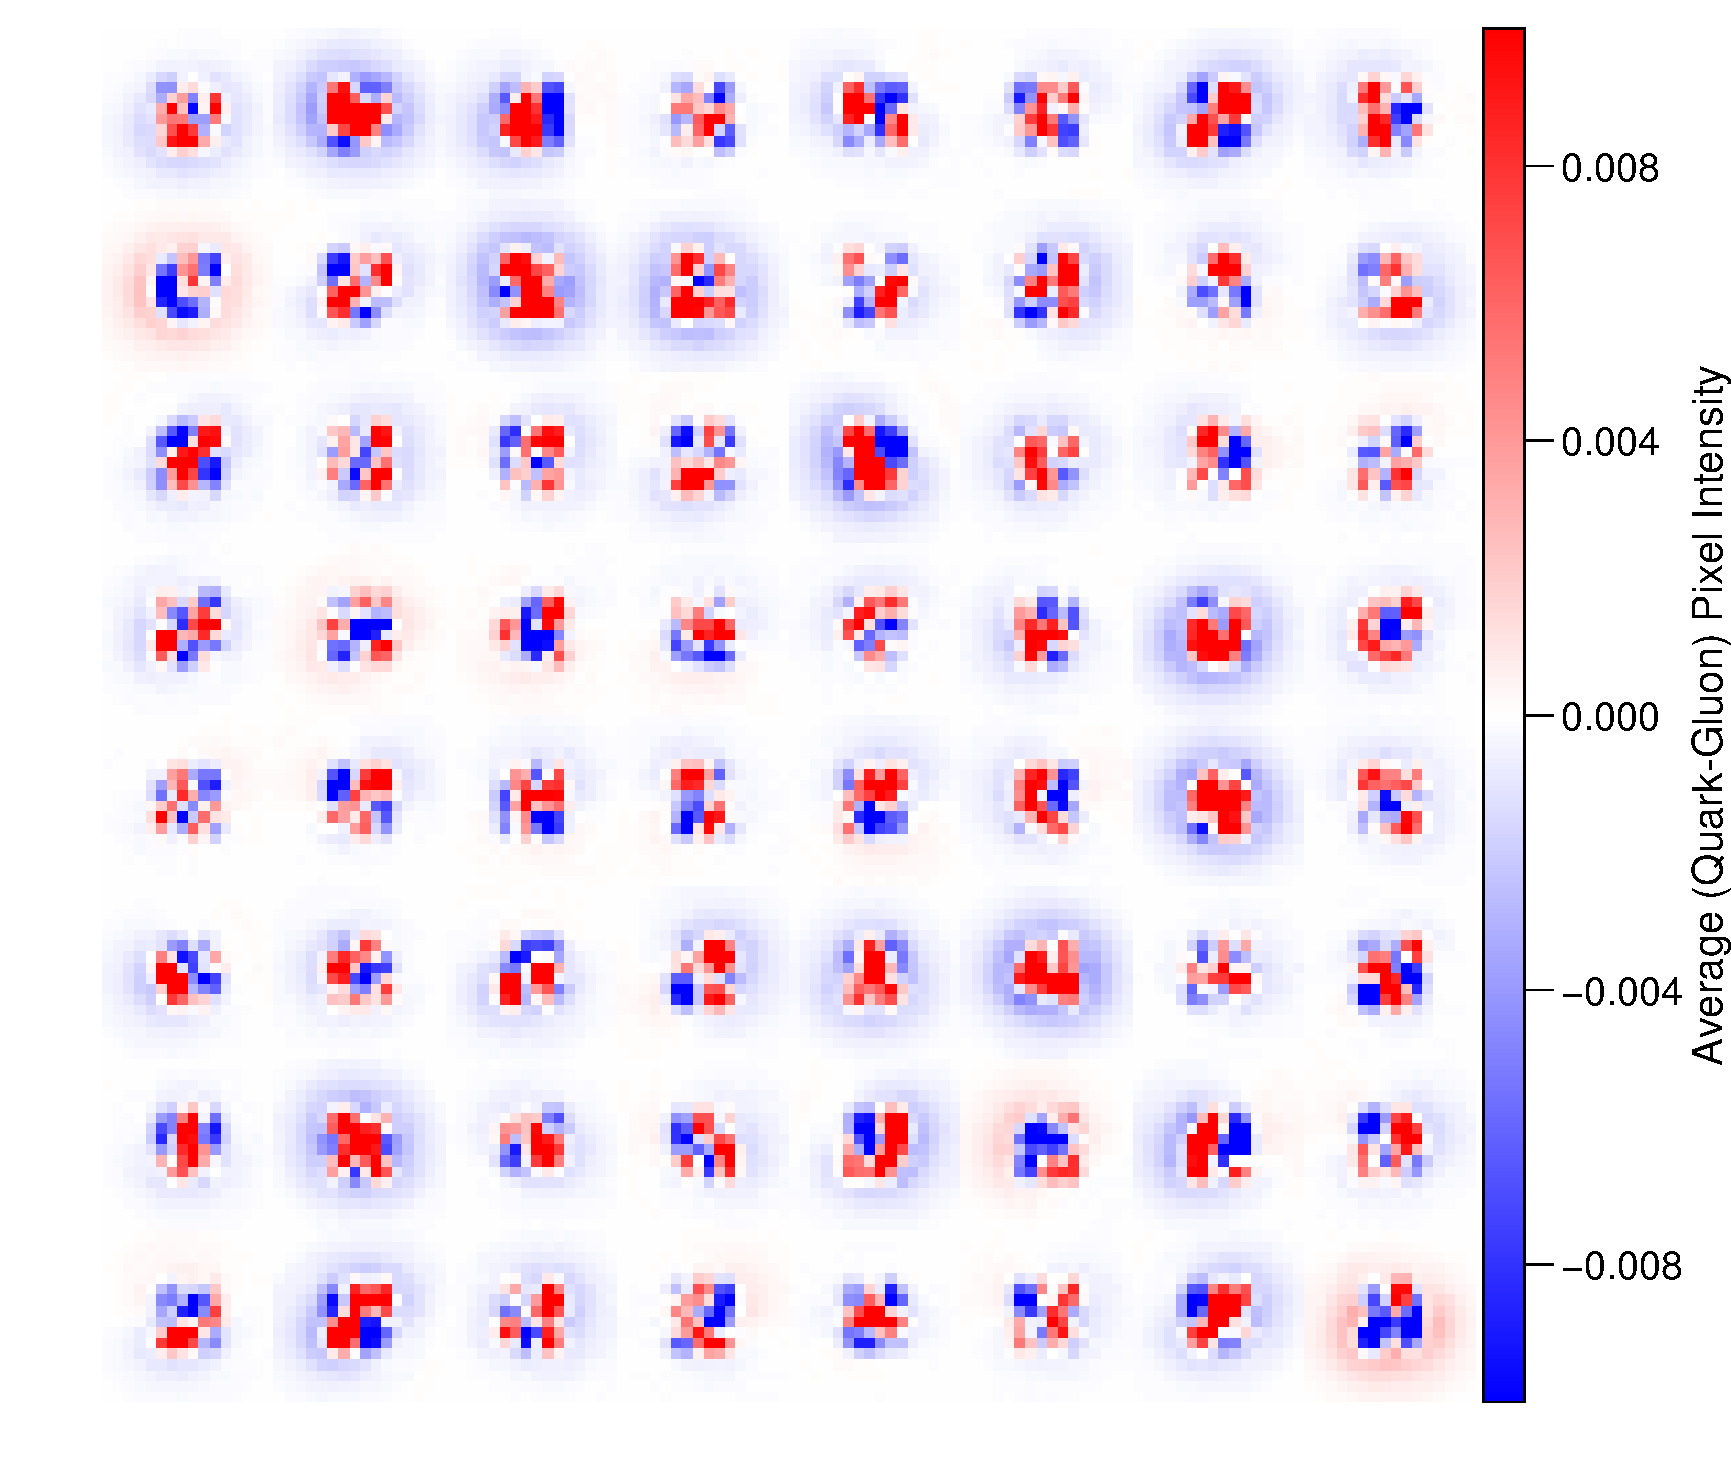
\includegraphics[width=0.9\textwidth]{figures/CNN/convimage_diff.pdf}}
\caption{
Average convolved filter differences for jet images (same color scheme as left plot; red is more quark-like). 
The filters of the first convolutional layer are considered.}
\label{fig:filters}
\end{center}
\end{figure}
